% Figure 1: intervals as points of the half-plane above the diagonal, and the first keys of Lex1 and Lex2.
% Compile with pdflatex; the PDF is included in main.tex at its natural size.
\documentclass[tikz,border=2pt]{standalone}
\usepackage[T1]{fontenc}
\usepackage{lmodern}
\usepackage{amsmath,amssymb}
\usetikzlibrary{arrows.meta}
\newcommand{\lo}[1]{\underline{#1}}
\newcommand{\up}[1]{\overline{#1}}
\newcommand{\K}{\mathcal{K}}
\definecolor{lattice}{HTML}{2A78D6}
\definecolor{lexb}{HTML}{EB6834}   % Lex2
\definecolor{lexa}{HTML}{1BAF7A}   % Lex1
\definecolor{ink}{HTML}{1A1A1A}
\definecolor{muted}{HTML}{6B6B6B}
\begin{document}
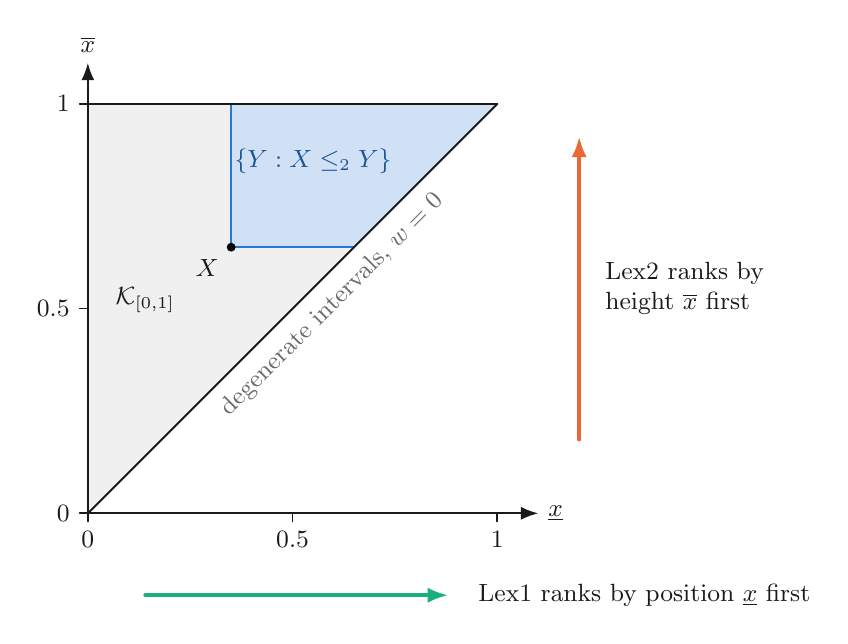
\begin{tikzpicture}[x=5.2cm,y=5.2cm,font=\small,text=ink,draw=ink,line cap=round]
  % the triangle K_[0,1]
  \fill[black!6] (0,0) -- (1,1) -- (0,1) -- cycle;
  % intervals above X in the product order
  \fill[lattice!22] (0.35,0.65) -- (0.65,0.65) -- (1,1) -- (0.35,1) -- cycle;
  \draw[lattice,line width=0.7pt] (0.35,1) -- (0.35,0.65) -- (0.65,0.65);
  \node[lattice!70!black] at (0.55,0.86) {$\{Y: X\le_2 Y\}$};
  \draw[line width=0.7pt] (0,0) -- (1,1);
  \draw[line width=0.7pt] (0,1) -- (1,1);
  \node[rotate=45,anchor=north,muted] at (0.56,0.545) {degenerate intervals, $w=0$};
  \node at (0.14,0.52) {$\K_{[0,1]}$};
  \fill (0.35,0.65) circle (1.6pt) node[below left=1pt] {$X$};
  % axes
  \draw[-{Latex[length=2.2mm]},line width=0.6pt] (0,0) -- (1.1,0) node[right] {$\lo x$};
  \draw[-{Latex[length=2.2mm]},line width=0.6pt] (0,0) -- (0,1.1) node[above] {$\up x$};
  \foreach \t in {0,0.5,1} {
    \draw[line width=0.6pt] (\t,0) -- (\t,-0.02) node[below] {$\t$};
    \draw[line width=0.6pt] (0,\t) -- (-0.02,\t) node[left] {$\t$};
  }
  % first keys of the two lexicographic orders
  \draw[-{Latex[length=2.6mm]},lexb,line width=1.3pt] (1.2,0.18) -- (1.2,0.92);
  \node[anchor=west,align=left] at (1.24,0.55) {Lex2 ranks by\\ height $\up x$ first};
  \draw[-{Latex[length=2.6mm]},lexa,line width=1.3pt] (0.14,-0.2) -- (0.88,-0.2);
  \node[anchor=west,align=left] at (0.93,-0.2) {Lex1 ranks by position $\lo x$ first};
\end{tikzpicture}
\end{document}
